\documentclass{article} % For LaTeX2e
\usepackage{url}
\usepackage[
style=authoryear,
backend=bibtex,
]{biblatex}
\usepackage{graphicx}
\graphicspath{ {../R_Code/Graphics/} }
\usepackage{enumitem}
\usepackage{placeins}
\usepackage{float}
\usepackage{multicol}
\usepackage{subfigure}

\addbibresource{ReportBib.bib}

\title{Final Report}
\author{
	Adam Dameron
}

\begin{document}
	
	
	\maketitle
	
	\begin{abstract}
		
	\end{abstract}
	
	\section{Demographic Transition}
	
	\section{Outline Methods}
	
	- Dataset (History, purpose, etc)\\
	- Types of models created\\
		- Why models require complete data and fewer variables (over fitting, computing power, etc)
	
	
	\section{Introduce Dataset}
	
	- Summarize dataset and define variables (https://cran.r-project.org/web/packages/naniar/vignettes/getting-started-w-naniar.html)\\
	- Explain what NA means in relation to the data set, and reasons NA may be present
	- Briefly describe/define missing (or complete) entries and explain why this matters\\
	- Remind that model can only be created with the complete entries\\
	
	\newpage
	\section{Manipulating CTDC Dataset}
	

	
	The CTDC data set contains 63 variables and 0 of its entries are complete. This means that without any data manipulation, creating a model is impossible. Creating a model is possible only if we have a significantly larger number of complete entries. One way to manipulate the data set into having a larger number of complete entries is by removing entire columns from the data set altogether. 
	
	While this process is efficient at creating complete entries, it is important to note that we would be losing some information in the process. For example, if we remove the variable that indicates if a victim was trafficking in the mining industry, then our final model cannot incorporate that information. This is why it is important a balance is struck between having complete entries, while still maintaining as much information as possible.
	
	Carefully choosing which variables to remove will help ensure we are aware of what information we are losing, and that will be accounted for that in the analysis of the final model. There are two ways in which variables (columns) will be omitted from the data set. The first way is by analyzing what the variable represents. By understanding what the variable means, we can logically conclude if it will be helpful, or if it should be removed. A second approach is to quantify the amount of incomplete entries that are caused by the variable, or a group of variables. By looking at missing values, we can see what variables are missing in tandem with each other. This would help us to better understand the structure of the data set, and provide a better understanding of what causes the missing values to appear.
	
	
	
	\subsection{Logically Removing Variables}
	 
	
	There are two variables that can be identified in the data set that meet this criteria. These variables are "Data Source" and "Year Of Registration." Both of these variables are representative of the manner and time in which a case was added to the data set. Data source is whether the case was reported over a hot line managed by IOM, or through a case manager on the victim's behalf. The year of registration is the year in which a case was added to the data set. Since these two variables only describe the reporting process, they will not be helpful in the process of identifying victims within a country, and can be removed without having a negative impact on the effectiveness of any models.
	
	A second type of variable that can be removed are those which serve to summarize other data contained within the data set. There are a few examples of variables which are concatenated versions of other variables and provide a written text summary. These variables are:
	
	\begin{multicols}{2}
		\begin{itemize}
			\item Means of Control Concatenated
			\item Type of Exploit Concatenated
			\item Type of Labour Concatenated
			\item Recruiter Relationship
		\end{itemize}
	\end{multicols}
	
	In a similar category as the previous variables, the "Majority Status" variable serves to identify whether or not a victim was an adult at the time they were exploited. However, the "Age Broad" variable already covers age information, and including "Majority Status" would essentially serve as a summary variable of the age information. While it is true that the age of majority is different in various countries, the Age Broad variable is a more specific representation of the characteristics of the victim.
	
	As a result of these findings, the following variables will be removed:
	
	\begin{multicols}{2}
		\begin{itemize}
		\item Data Source
		\item Year Of Registration
		\item Means of Control Concatenated
		\item Type of Exploit Concatenated
		\item Type of Labour Concatenated
		\item Recruiter Relationship
		\item Majority Status
		\item Majority Status at Exploit
		\item Majority Entry
	\end{itemize}
	\end{multicols}
	
	After removing these columns, our data set now has 590 complete cases. This is an improvement, but it is certainly not enough to make any meaningful model. However, quantitative methods will yield better results.

	
	\subsection{Quantitatively Removing Variables}
	
	The second way that individual variables can be removed is by using quantitative methods. There are many processes to complete this task, and a handful of them will be applied to this data set. 
	
	One way is to simply look at all the different values that the variable takes. If we see that all the entries for a variable in the data set are either NA or 1, then it is clear that any complete row will have a value of 1 for that variable. This means that the model will only take in the value of 1 for that feature in each row. Thus the variable will have a null effect on the model. This process led to the removal of:
	

	\begin{multicols}{2}
		\begin{itemize}
			\item Is Forced Military
			\item Is Organ Removal
			\item Type of Labour Mining/Drilling
		\end{itemize}
	\end{multicols}
	
	After removing these variables, there are still only 590 complete entries. However, the removal of these variables can do nothing but help us, as there is no way they can have an effect on our model. Unfortunately, these variables are the only type that we can remove and have no negative consequences. Any other variables we omit will have downsides, and it would be beneficial to try to find which variables are having a significant effect on the number of missing values, and to remove those. Since each absent entry is given a value of NA, we can count the number of NA's in each column to get a sense of which ones are contributing the most to the lack of complete entries.
	
	\begin{figure}[H]
		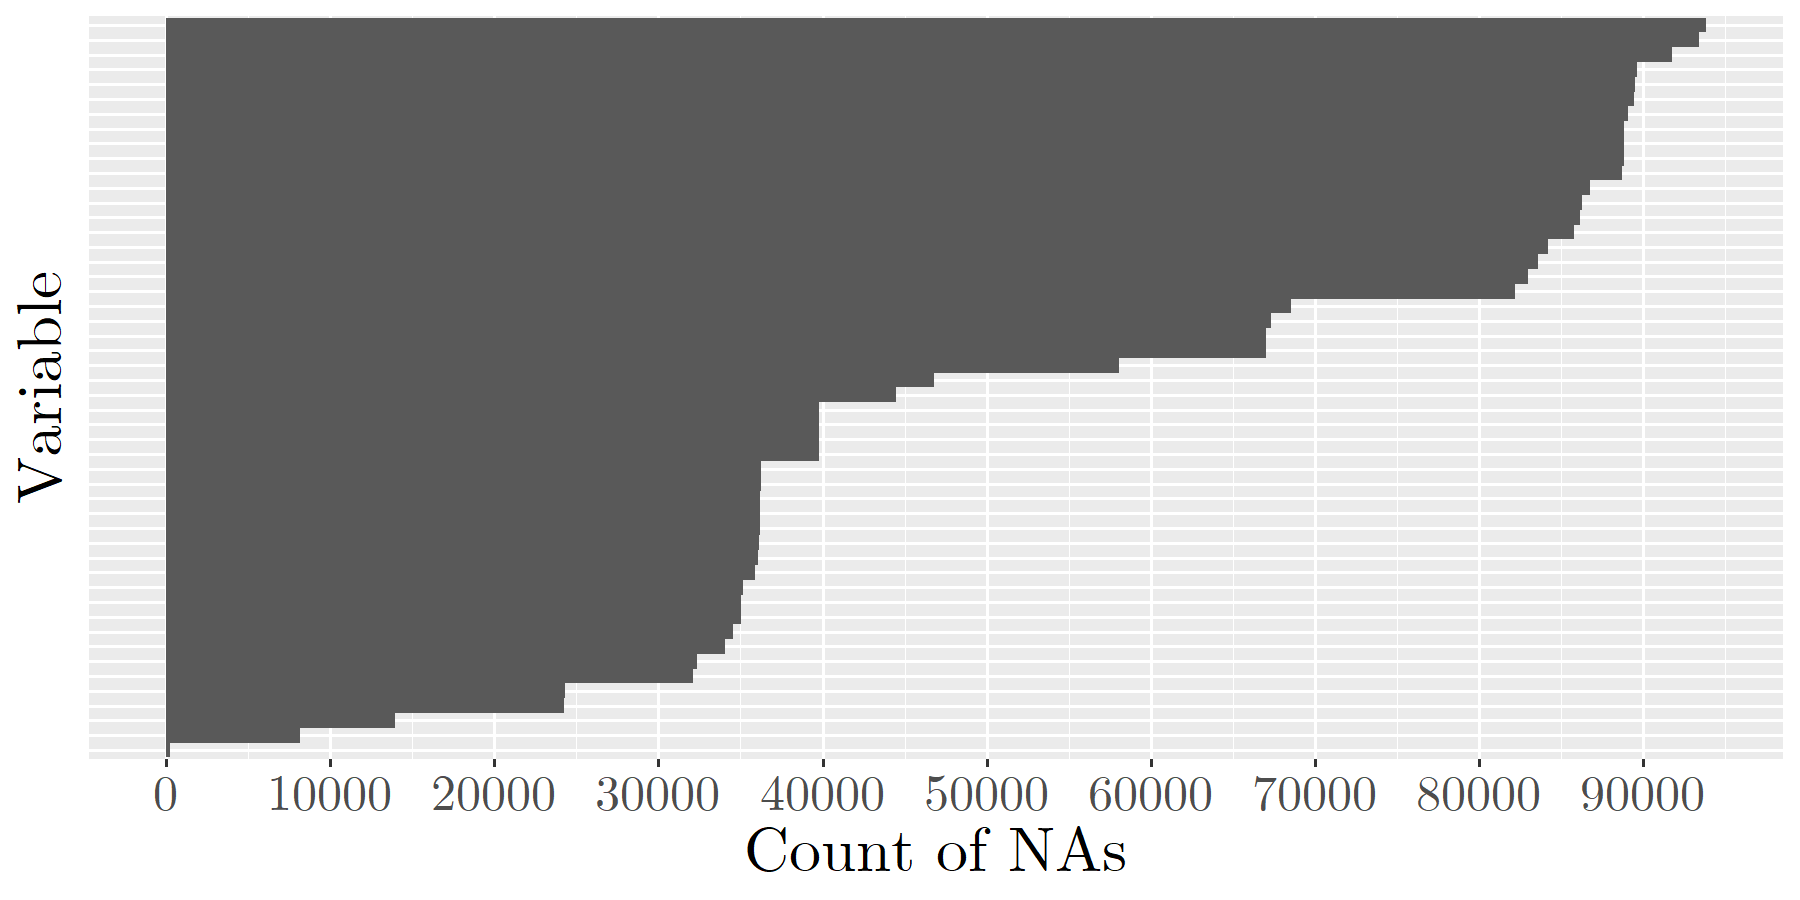
\includegraphics[width = \textwidth]{NABarplot}
	\end{figure}
	
	Given the large number of variables, the variable names have been omitted from the visual. However, some important information can still be gathered. One can see that every variable has at least a handful of missing values. As such, it would be helpful to start with the variables that have the highest count, and see if there are any patterns. There is a steep drop off of the count of NAs at around 75,000 (emphasized with red line), so analyzing all the variables with more than 75,000 NA could give some useful information.
	
	\begin{figure}[H]
		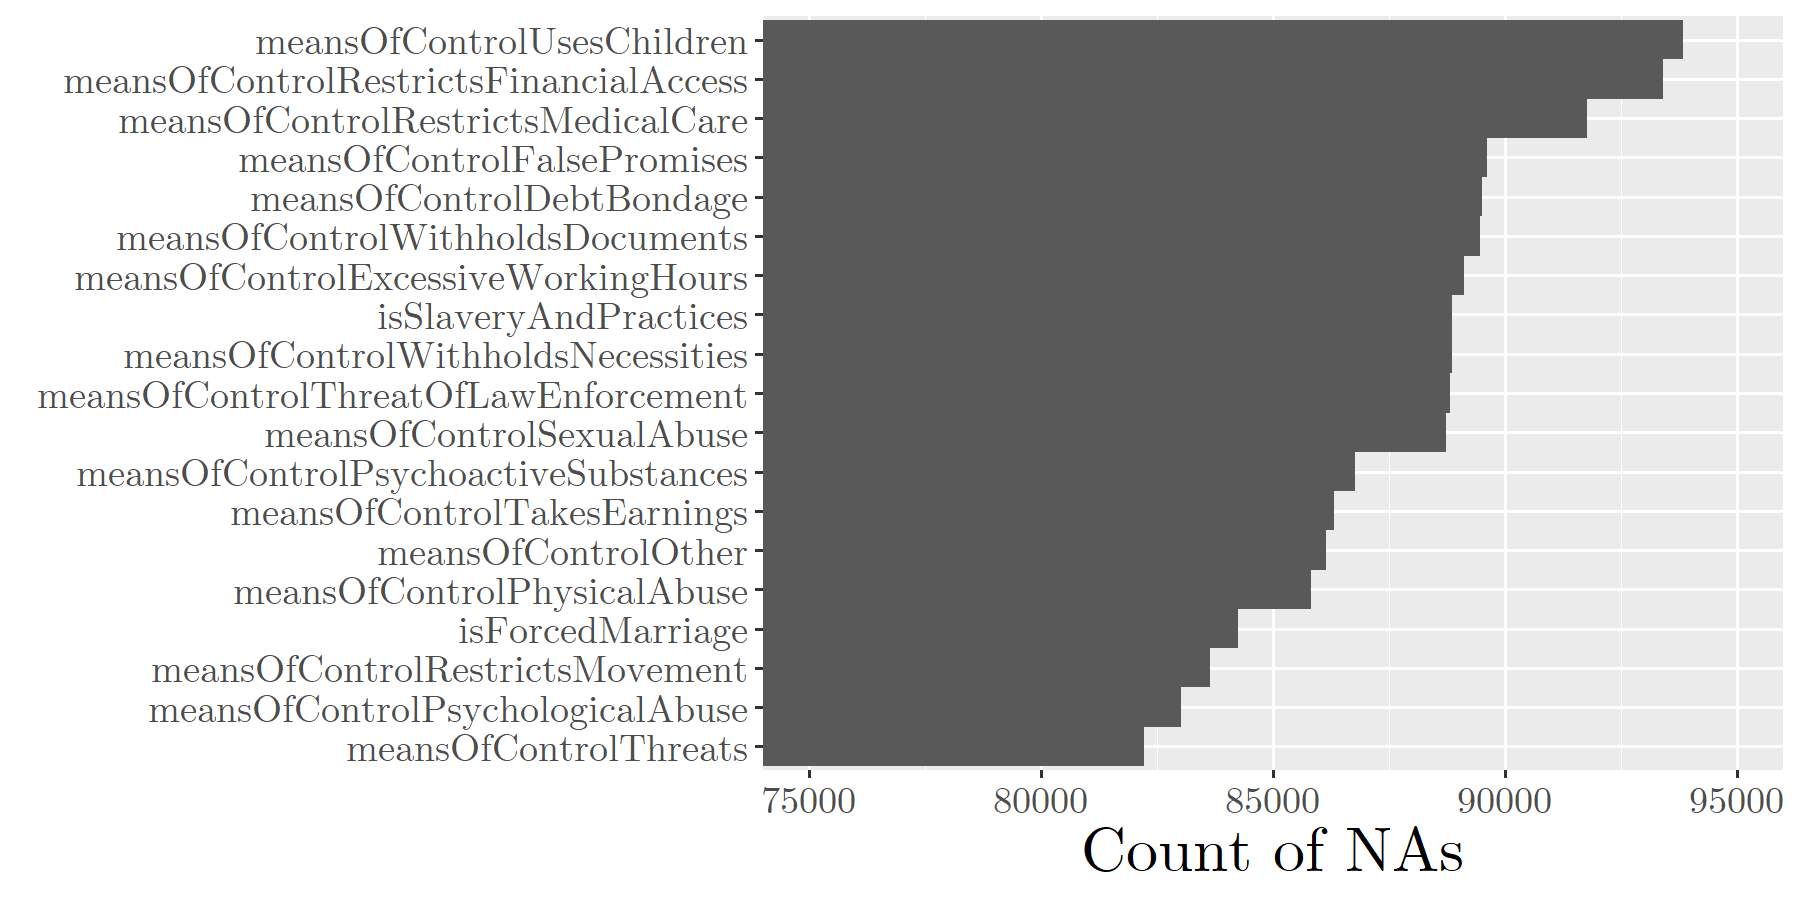
\includegraphics[width = \textwidth]{NABarplot2}
	\end{figure}
	
	From the figure, one can see that the "meansOfControl-" variables take up a large number of spaces on the list. Of the 19 variables with over 75,000 NA values, 17 of them are "meansOfControl-." This could be a direct effect of the way in which the data is recorded. If an individual is transcribing cases to the data set, they may have decided that after determining that one type of control was used, to leave all the other types as "missing." The data set does have a variable that is 1 if there is no specified means of control. We can analyze this variable to determine if it would be worthwhile to modify the data set to salvage the means of control information that does exist.
	
	The "means of control not specified" variable takes a value of 1 if there is no specified means of control. This variable has roughly 50,000 values of 1, and roughly 30,000 values of 0. Meaning that only 30,000 entries in our data set have a means of control specified. By replacing each NA in these variables with 0, we are able to add up all the values for each entry in the data set. This will tell us how many means of control variables are specified.
	
	\begin{figure}[H]
		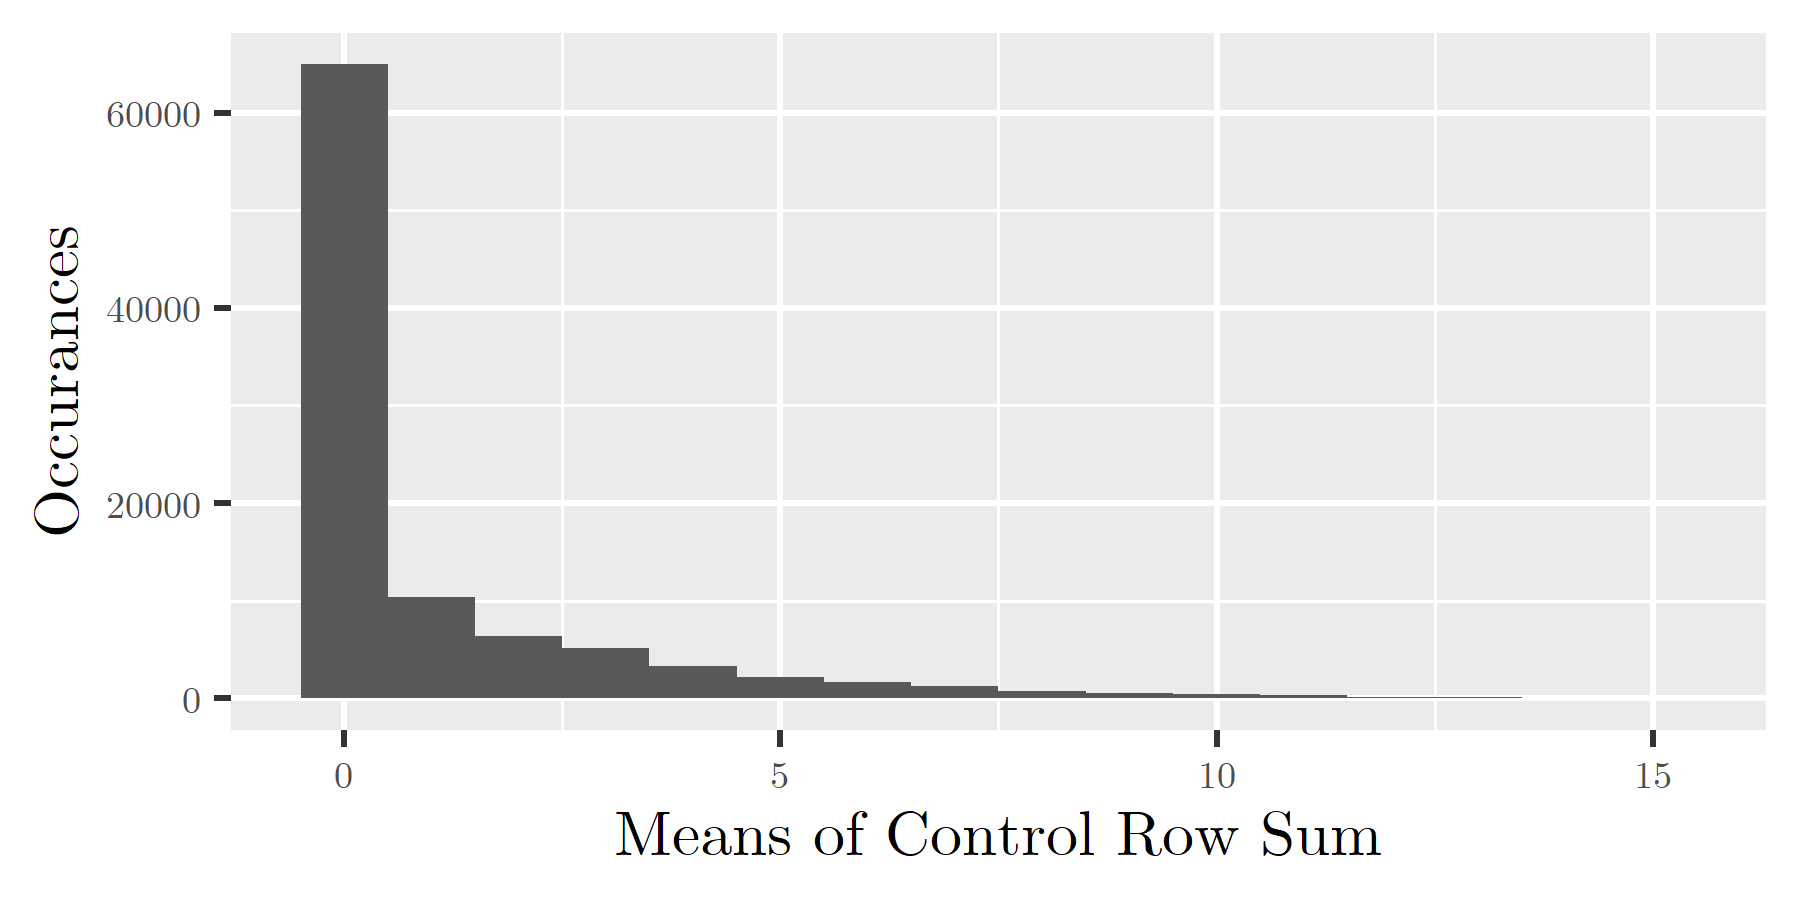
\includegraphics[width = \textwidth]{MeansOfControlSumHist}
	\end{figure}
	
	This histogram allows a visualization of how many instances there are of means of control not being specified. From this histogram, one can see that row sums of 0 are the most common and make up over two-thirds of the data entries. This means that a large proportion of our data cannot even be salvaged by replacing NAs with values of 0. Even if one were to choose to replace the NAs with 0, the sheer lack of recorded entries implies that this data is hard for law enforcement to notice. As such, even if these variables were considered to have a significant effect on model outcomes, there are so many of them that the model would place a higher importance on these types of variables. This is a result of over fitting, and since we want the final model to be applicable and easy to understand, removing these would lead to that goal the quickest.
	
	After removing the Means of Control variables, we are left with 33 variables, and 596 complete entries. This is great progress, but more can be made. To get a better idea of where missing values are, the following visualization is helpful:
	
	\FloatBarrier
	\begin{figure}[H]
		\hspace*{-2cm}
		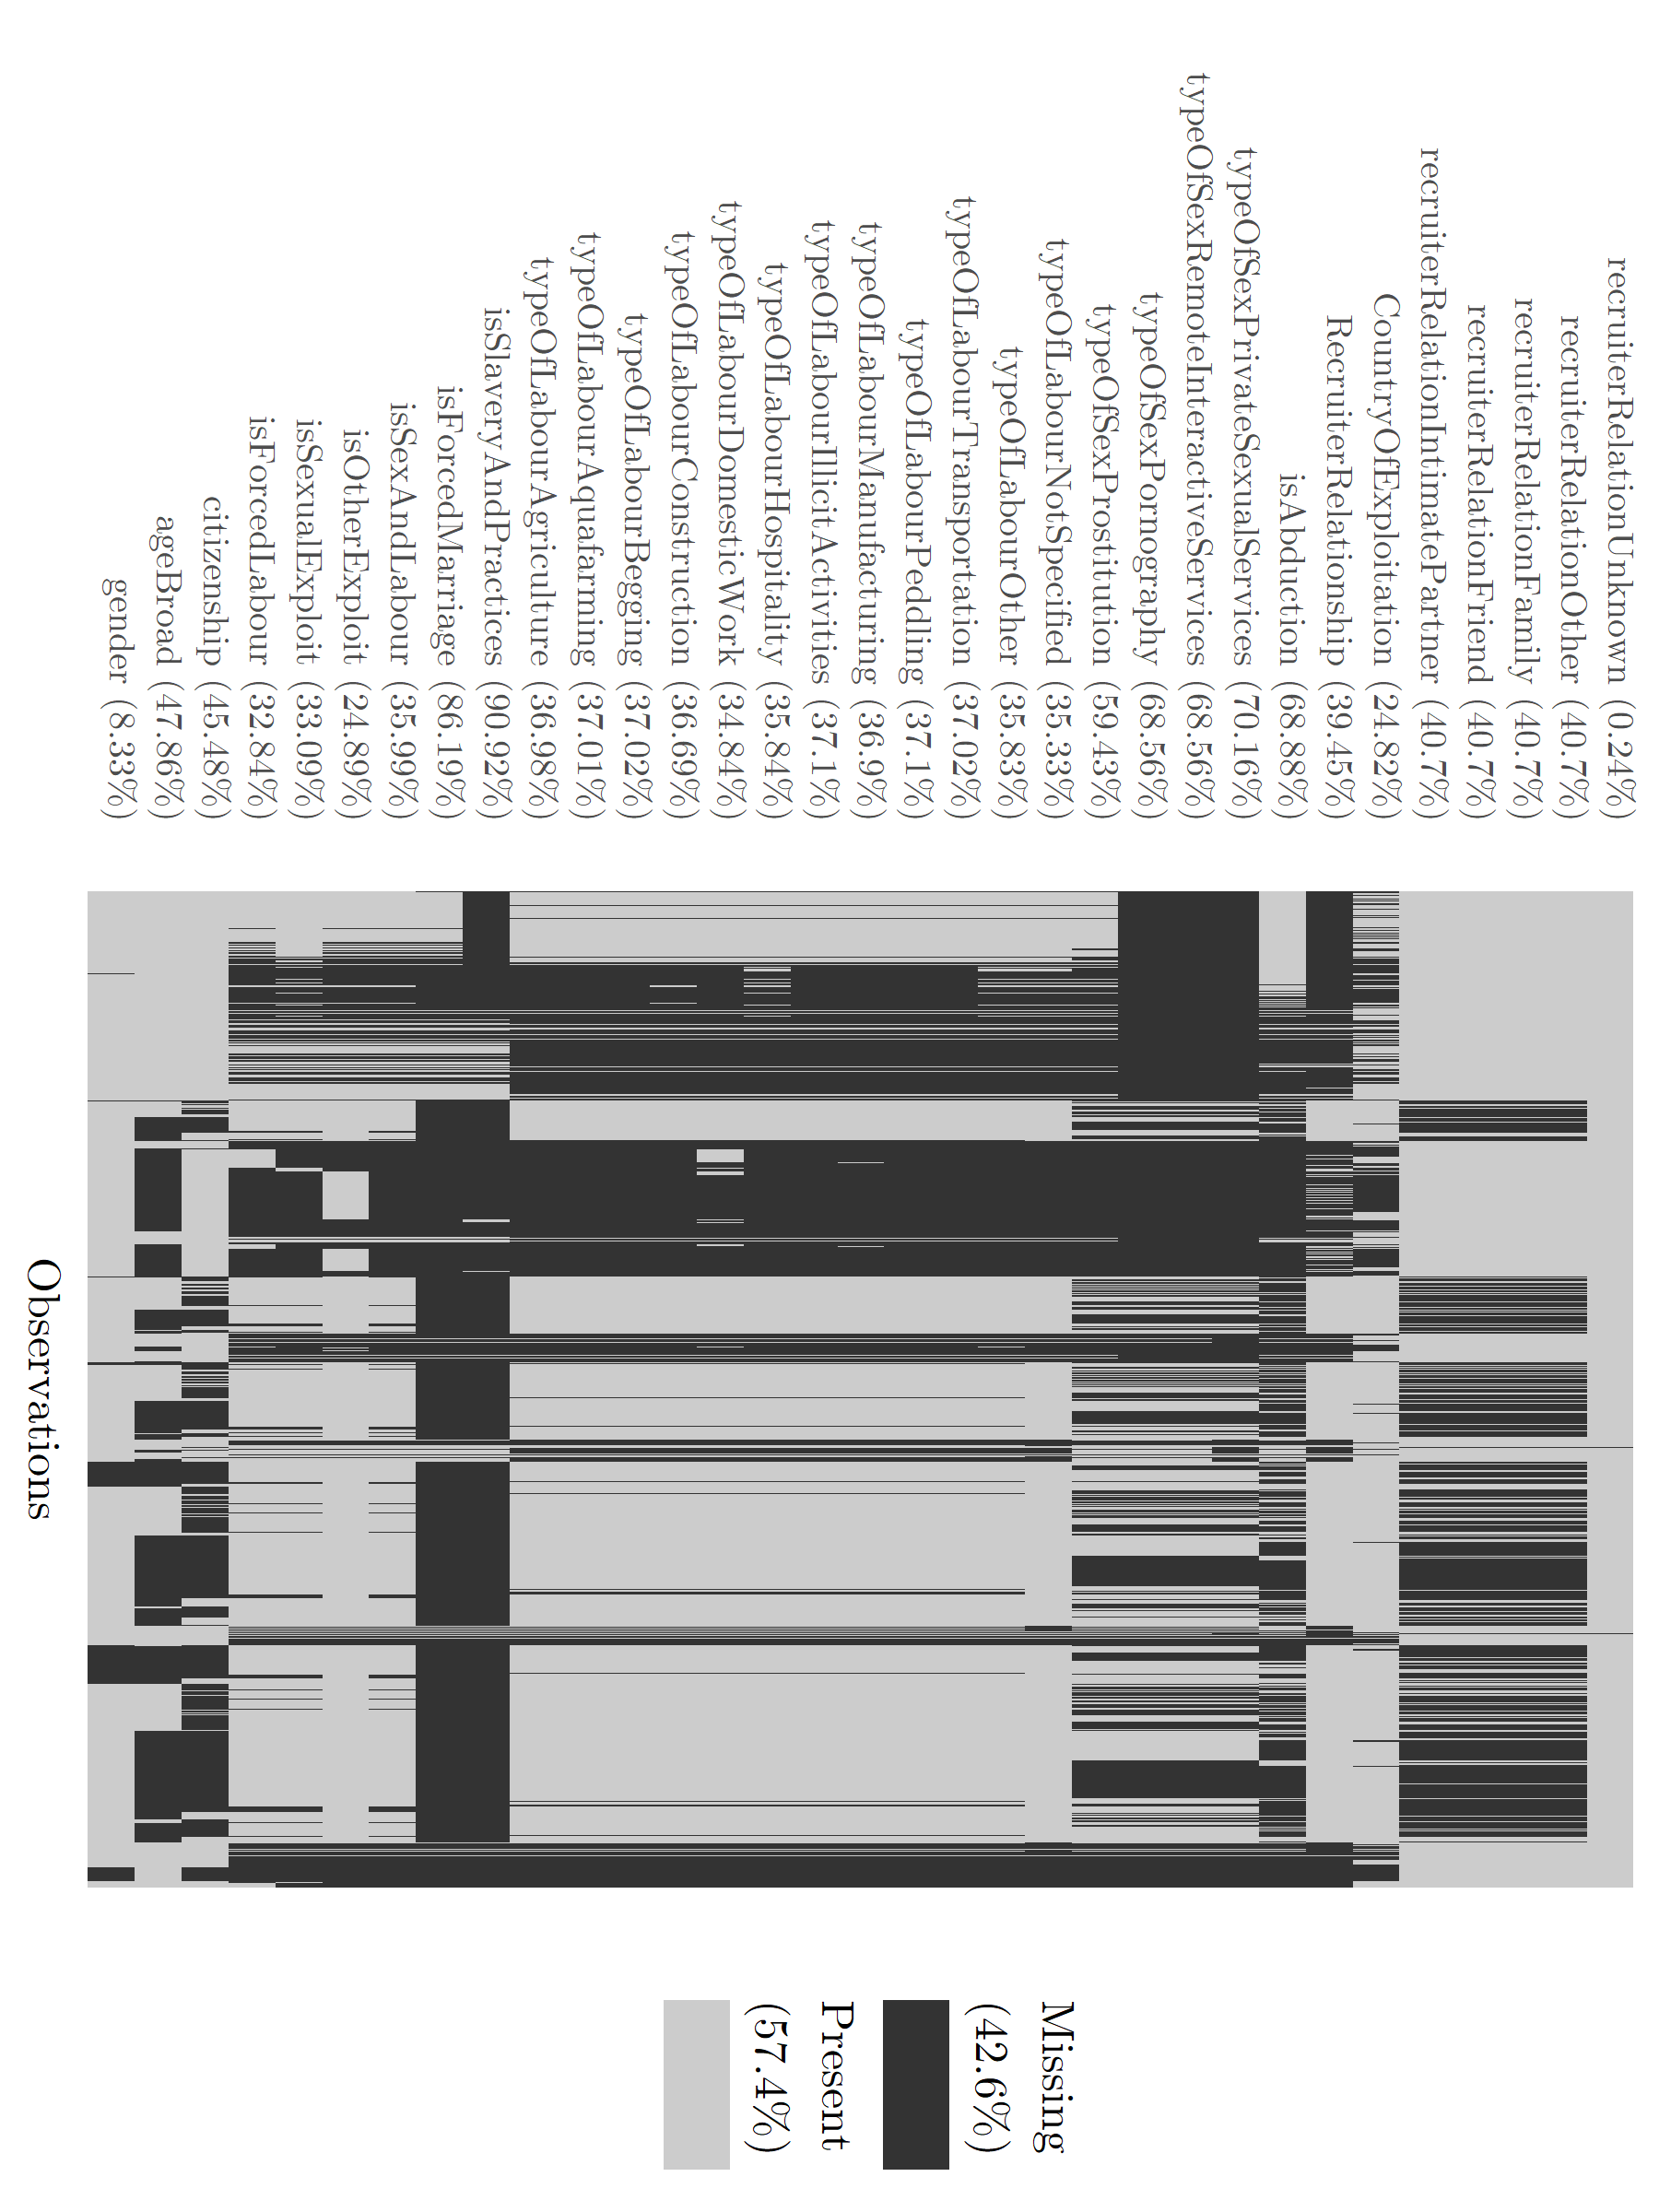
\includegraphics[height = 1.4\textwidth, angle = 90]{NaniarVis1}
	\end{figure}
	\FloatBarrier
In this visual, the missing values for each variable are shown visually. Each row in the visual represents a category in the data set, and the columns show each row. For example, we can see large bands of missing data in both the horizontal and vertical directions. Horizontal bands of missing data correspond to that variable having a lot of missings. For example, isSlaveryAndPractices is missing 90.92\% of its values, and as such that row seems to be almost entirely black. 

Additionally, there are instances when there seems to be a large correlation between values missing in different variables. An example of this would be the "recruiter relation" variables. In virtually all cases in which one of these variables is missing, all the others are missing as well. This is interesting, as it would imply that if the recruiter relation was known, values of 0 were entered for the recruiter relationships that were not present. This is contrast to the means of control variables, in which NA was evtered even if another means of control was observed. This leads one to believe that there is inconsistent data entry practices within the IOM.

From this visual, we would consider removing "isSlaveryAndPractices", and "isForcedMarriage", as they have percentages of missing values, 90\% and 86\% respectively, that are significantly higher than the other variables. Removing these variables brings the number of complete entries from 596 to 1,218 complete cases. Removing these two variables has more than doubled our number of complete entries.

While 1,218 is enough complete entries to create some meaningful models, it is still only representative of less than 2\% of all the entries in the data set. It would be a good idea to look at some interactions between missing variables, to see if there are any that are missing together as opposed to individually. This can be done with an Upset Plot, as is outlined in \cite{UpsetPlot}.

\begin{figure}[H]
	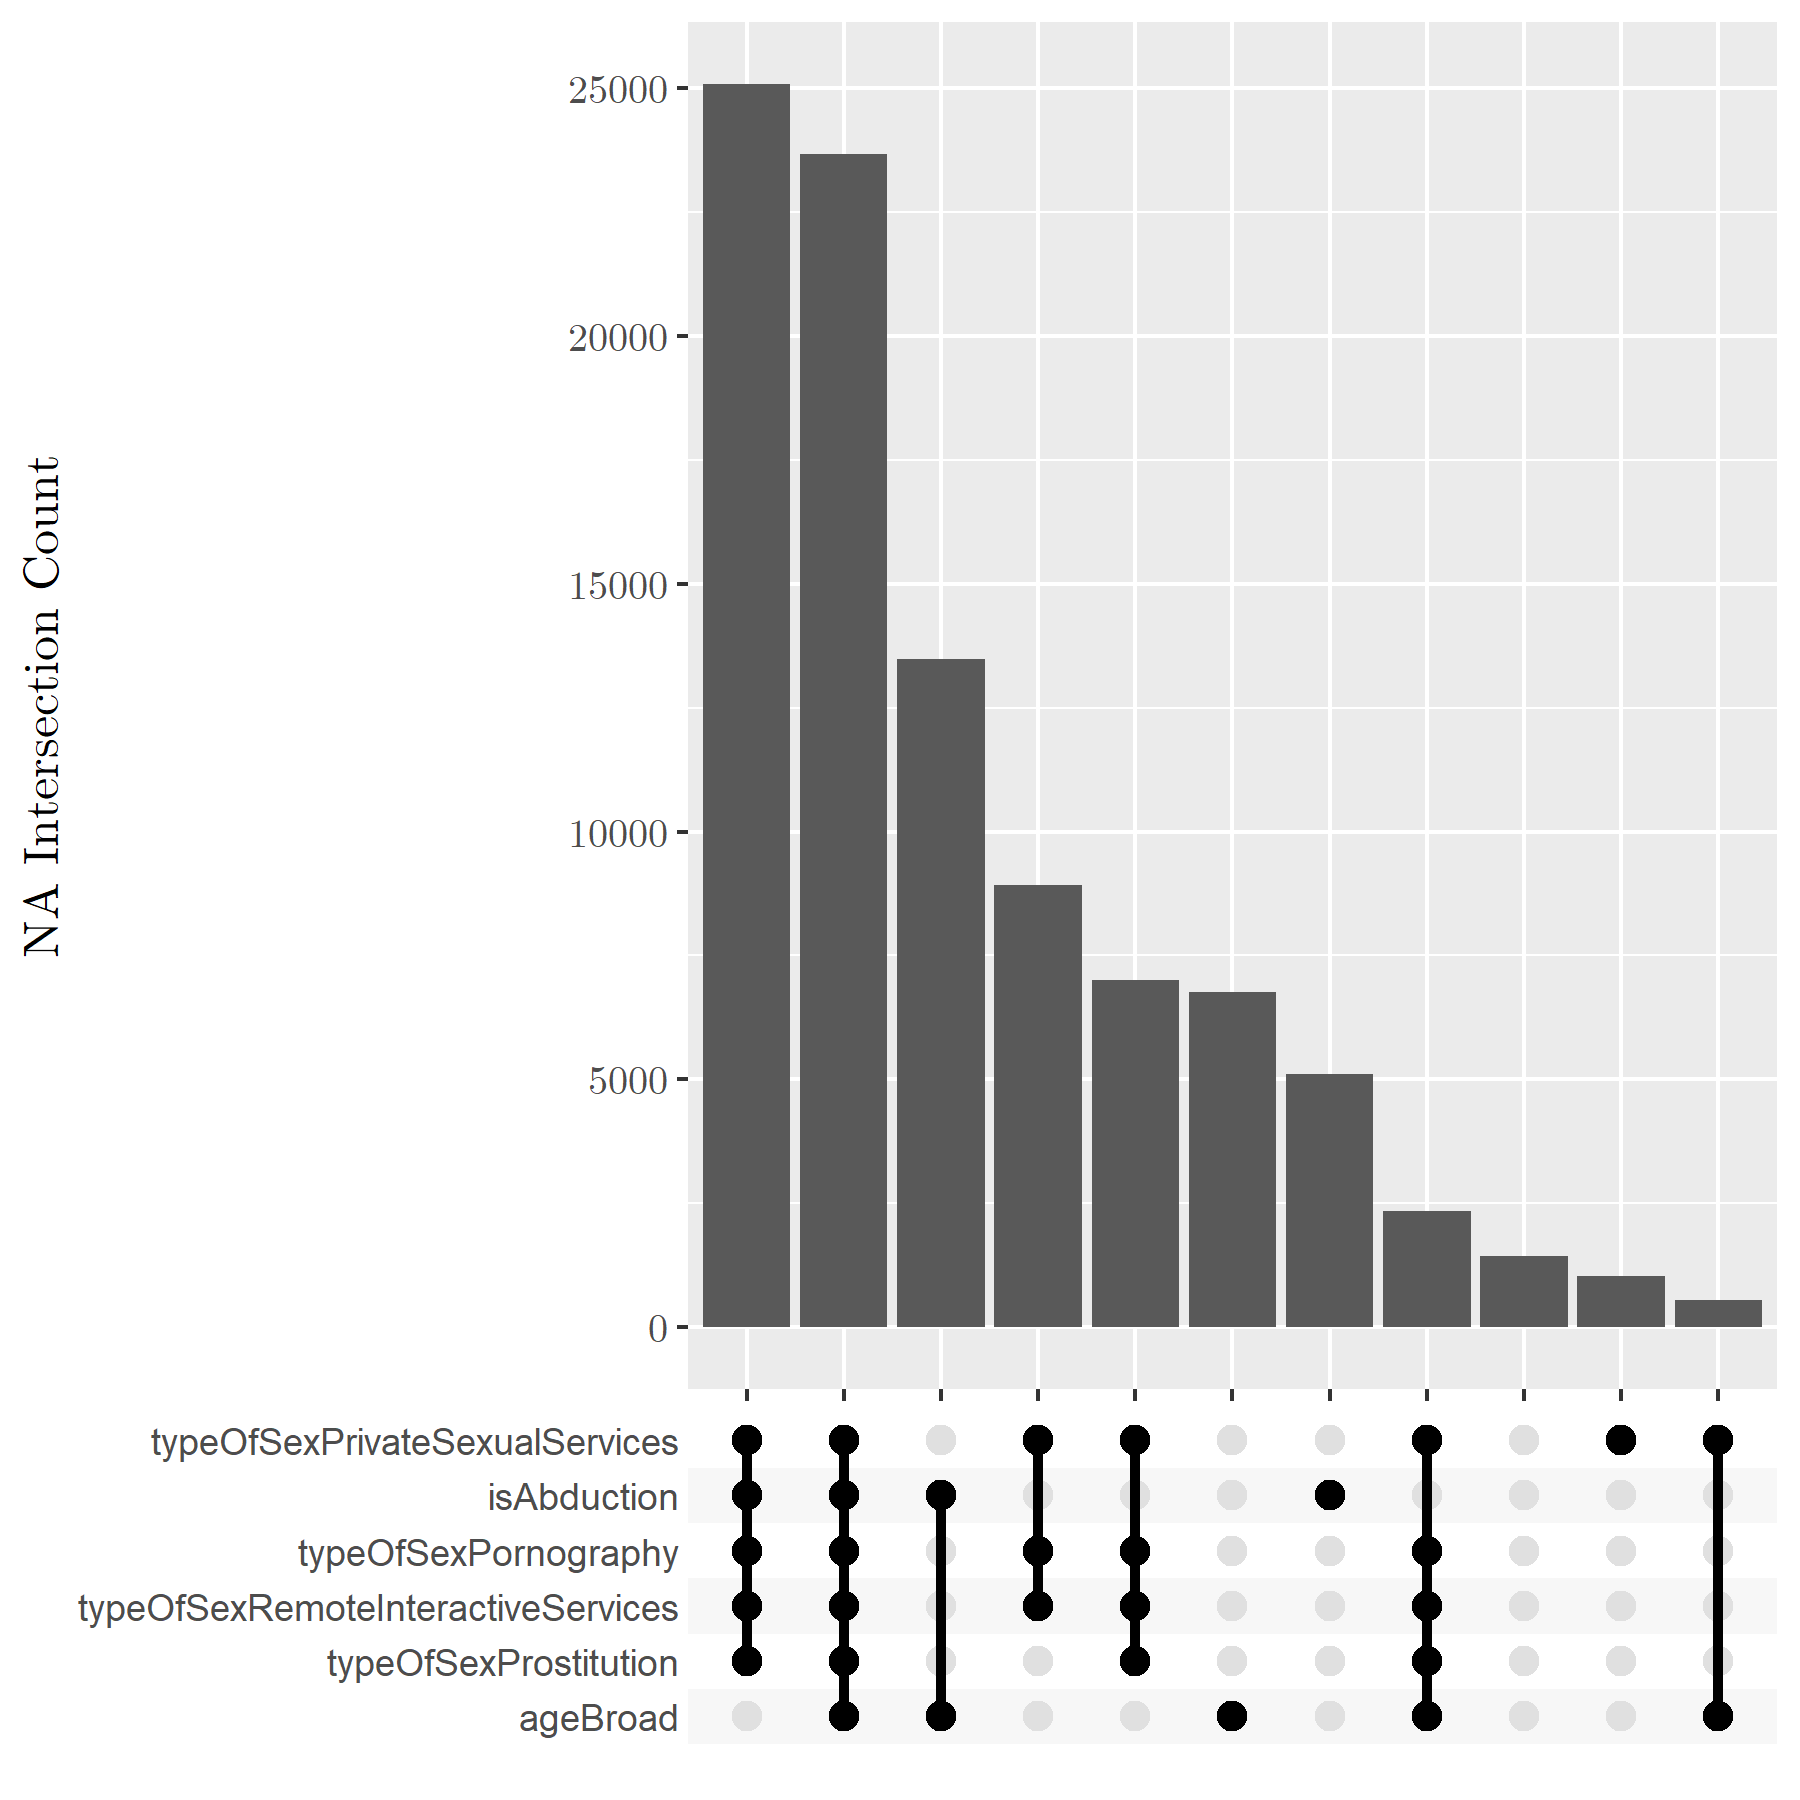
\includegraphics[width = \textwidth]{UpsetPlt1}
\end{figure}

From this visualization, along the bottom, one can see which sets of variables lead to the most missing values. For example, the "type of sex" variables and "isAbduction" have a count of roughly 25,000. This means that there are 25,000 rows in our data set that are missing all of those values. This gives us a visual way to determine which variables contribute to incomplete entries, and give us the exact number of rows that are incomplete due to those combinations of variables. Thus, we can attempt to find groups of variables that have a high number of missing rows, but that we also feel would be ineffective metrics that alw enforcement and policy makers can use. 

The first set of variables have over 25,000 incomplete rows; however, removing 4 variables seems like it would be too much, especially since tis group includes "isProstitution" and "isAbduction," both of which are variables that have been shown to be correlated with high rates of human trafficking \parencite{SlaveBook, polarisTypology}. The first set that does not contain either of these two variables is set 4, which contains private sexual services, pornography, and remote interactive services. These are variables that one can feel comfortable removing, as they contribute to a large number of incomplete rows, and are hard to find and prevent from a law enforcement and policy perspective.

Removing these variables yields 2950 complete cases with 28 total variables. While this process did not take into account the root causes for missing data, later discussion will attempt to determine these causes, and explain what effect it has on the final model. At this point, there are a large enough number of complete entries with a small count of variables, enough for the modeling process to begin.

\subsection{Augmenting Demographic Transition Data}

As previously mentioned, a country's stage in demographic transition can be determined by looking at a current population pyramid for that country. To accomplish this, the United States Census Bureau has publicly available data of every country \parencite{USCB}, including current population pyramids. By observing these, one can determine a country's current stage in demographic transition. This information was then appended to the CTDC Data Set and will serve as the dependent variable in this research. These values will replace country names in the "citizenship" and "CountryOfExploitation" variables.

\subsection{Final Removal}

After all the changes made, there are now more colomns in which every value is the same. Naturally, these columns will be removed from the data set, but the number of complete entries will remain he same. These variables are:

\begin{itemize}
	\item Type Of Labour Illicit Activities
	\item Type Of Labour Peddling	
	\item Type Of Labour Transportation
	\item Type Of Labour Not Specified
	\item Is Abduction		
\end{itemize}

\newpage
\section{Preliminary Data Analysis}

Before creating any models, some initial analysis of our current data set would be useful. Looking at any trends that may already exist will prove to be useful in the model creation process.

\subsection{DTM Stages Data}

\FloatBarrier
\begin{figure}[H]
	\subfigure{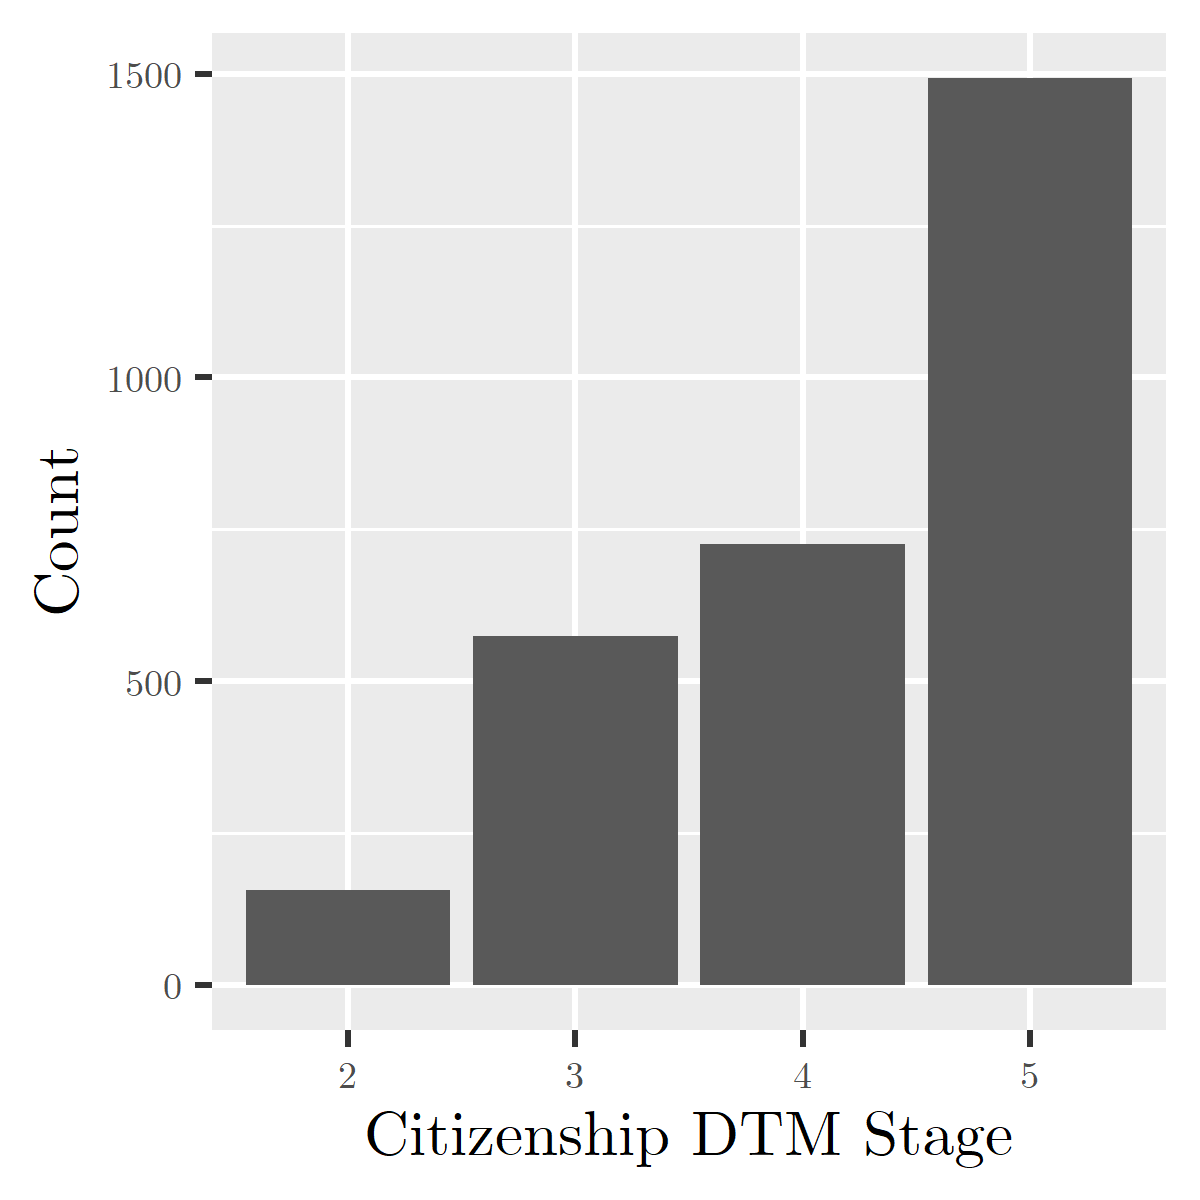
\includegraphics[width=0.491\textwidth]{CitDTM}}
	\subfigure{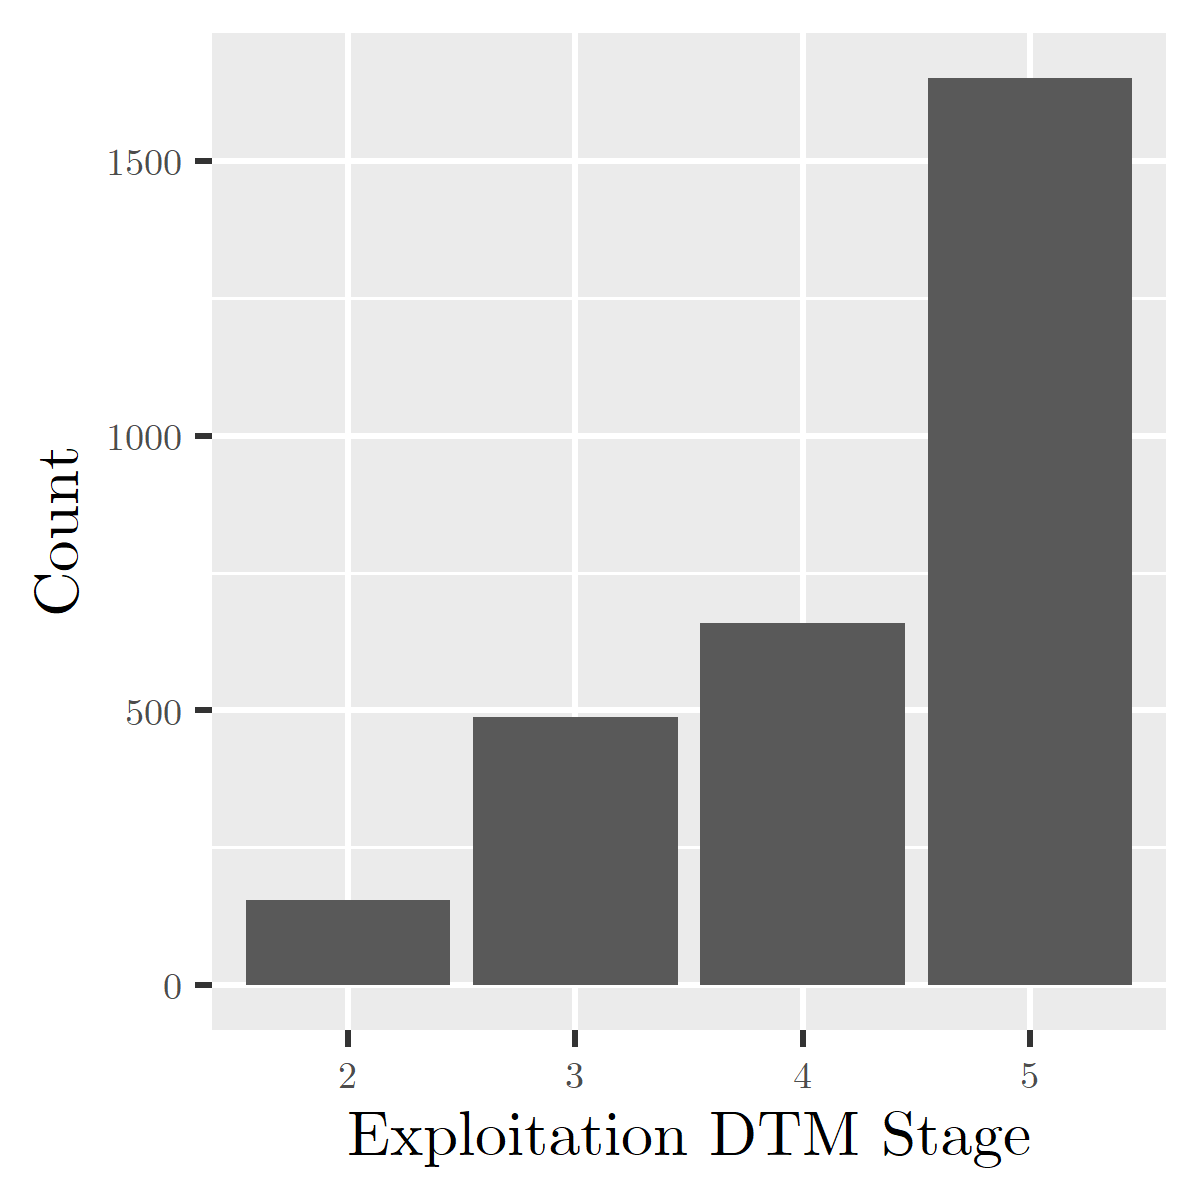
\includegraphics[width=0.491\textwidth]{ExpDTM}}
\end{figure}
\FloatBarrier

In this graphic, one can see that the majority of entries for Citizenship and Exploitation DTM are stage 5, with a decreasing count as the stage decreases. This certainly is interesting, but is something one would expect to see for the DTM stage of exploitation countries. Since these are typically the places in which the victim's case is recorded and added to the CTDC data set, this is not abnormal. One would expect more developed countries to have higher rates of reported cases, as they have access to the resources required to locate the victims. However, this does not explain the trend in Citizenship DTM Stages.

\FloatBarrier
\begin{figure}[H]
	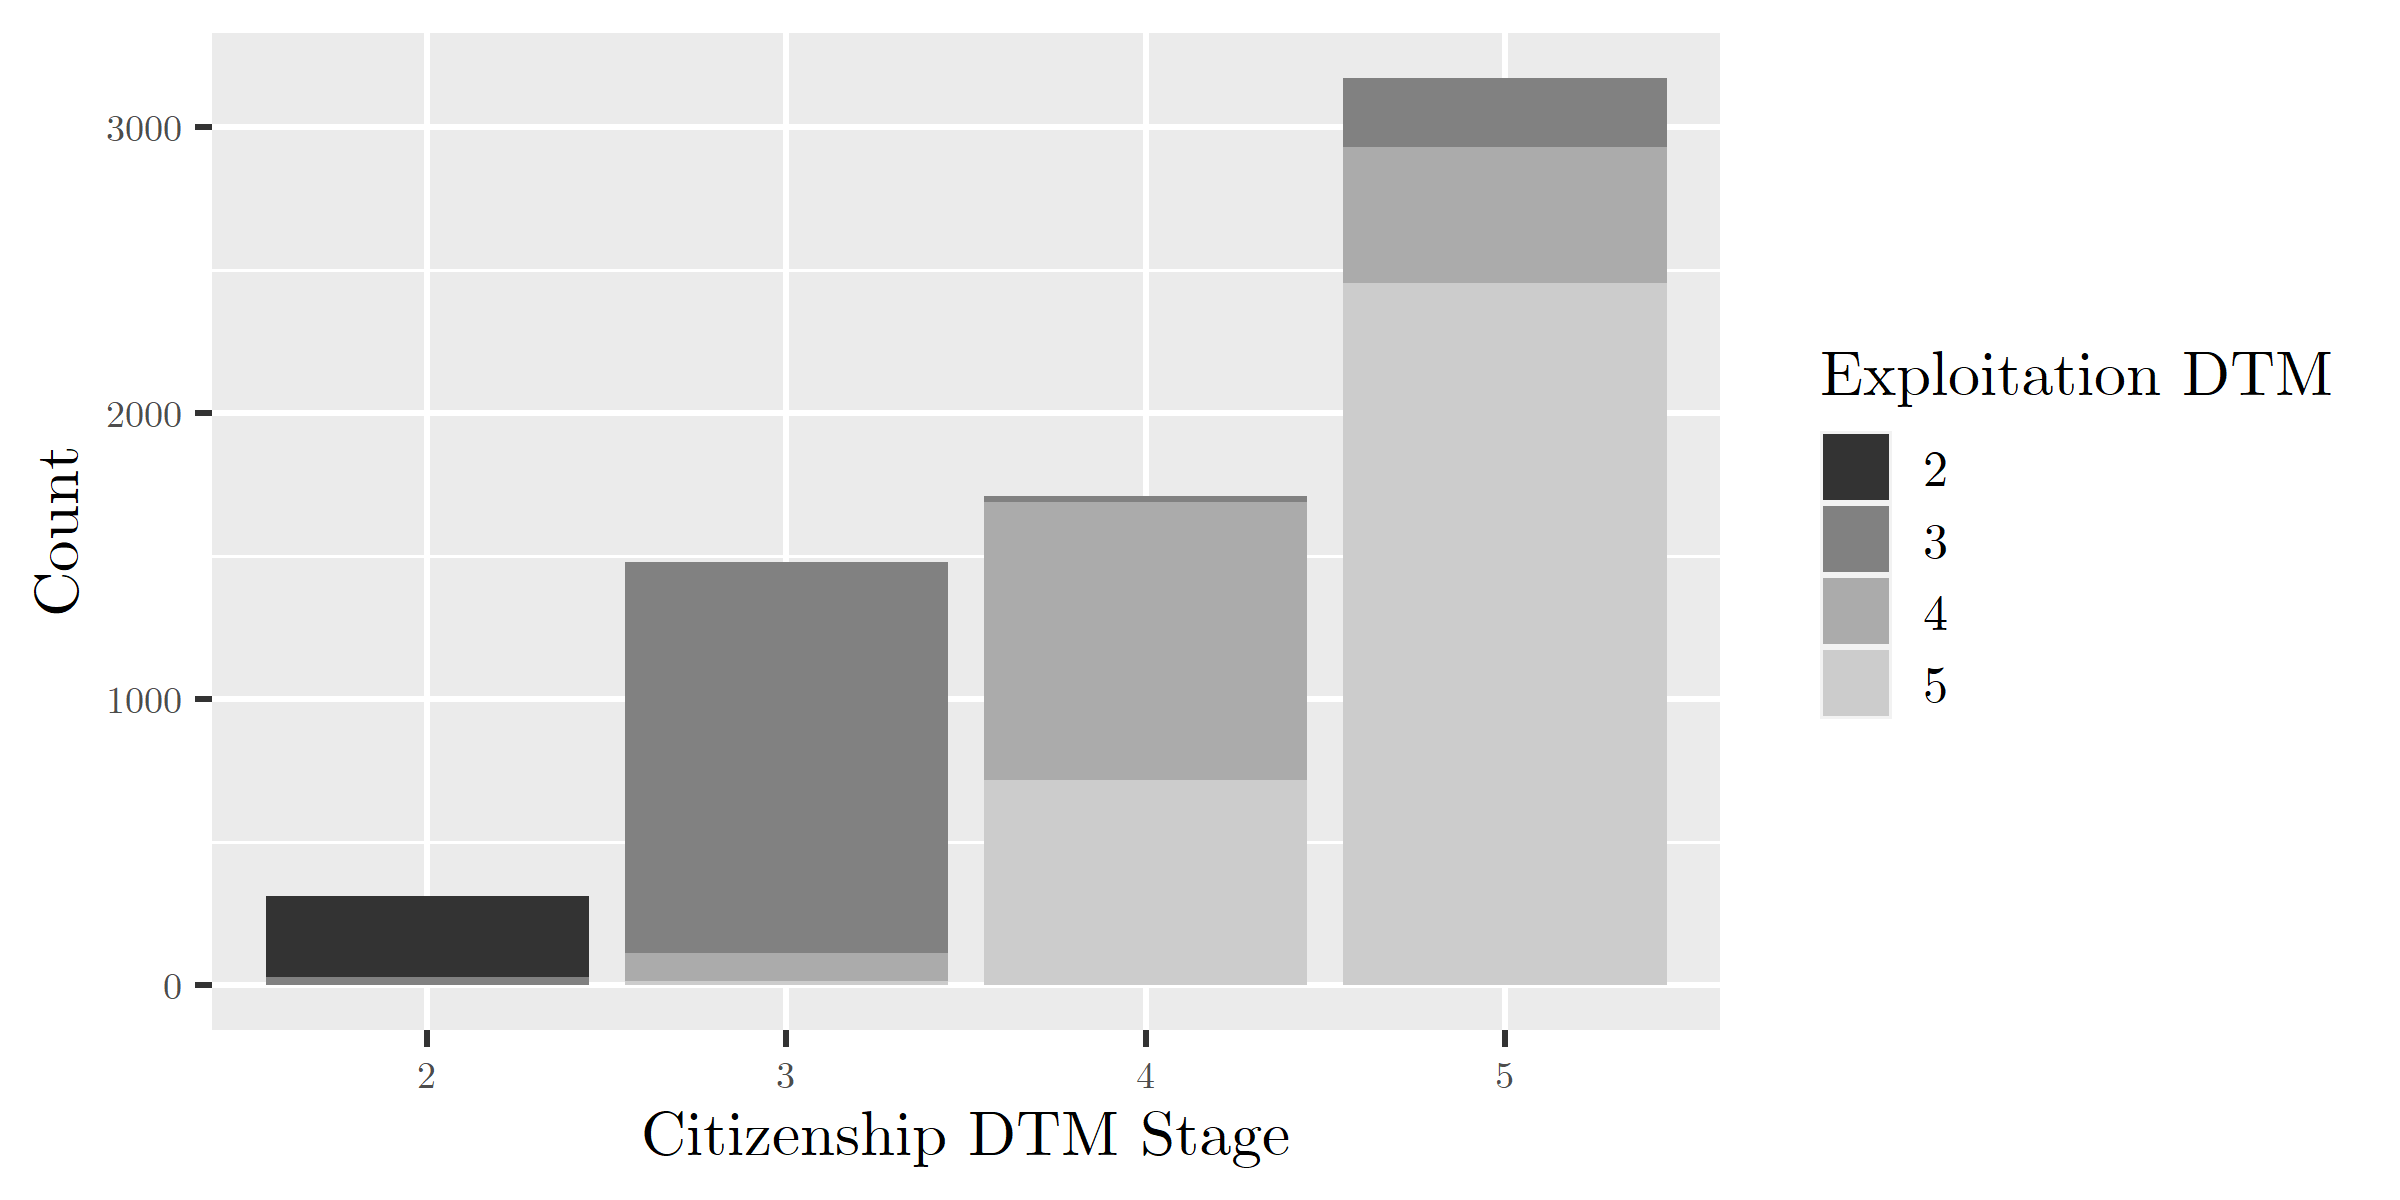
\includegraphics[width = \textwidth]{DTMStage1}
\end{figure}
\FloatBarrier

From this chart, one can see the intersection of the two plots. Each bar has the total count of entries with a certain citizenship DTM stage, and each bar is broken down into the counts of the exploitation DTM stage. For example, one can see that there are roughly 500 victims with a citizenship DTM stage of 3, and of those, the majority are exploited in a country that is also stage 3.

Of interest in this chart is the fact that for every citizenship DTM stage, the majority of the victims are exploited in a country of the same stage. This pattern can easily be explained by victims typically being exploited in their citizenship country. Further analysis shows that 777 of the 2950 entries (26.3\%) are examples of this. When we remove these entries, the visualization looks like this:

\FloatBarrier
\begin{figure}[H]
	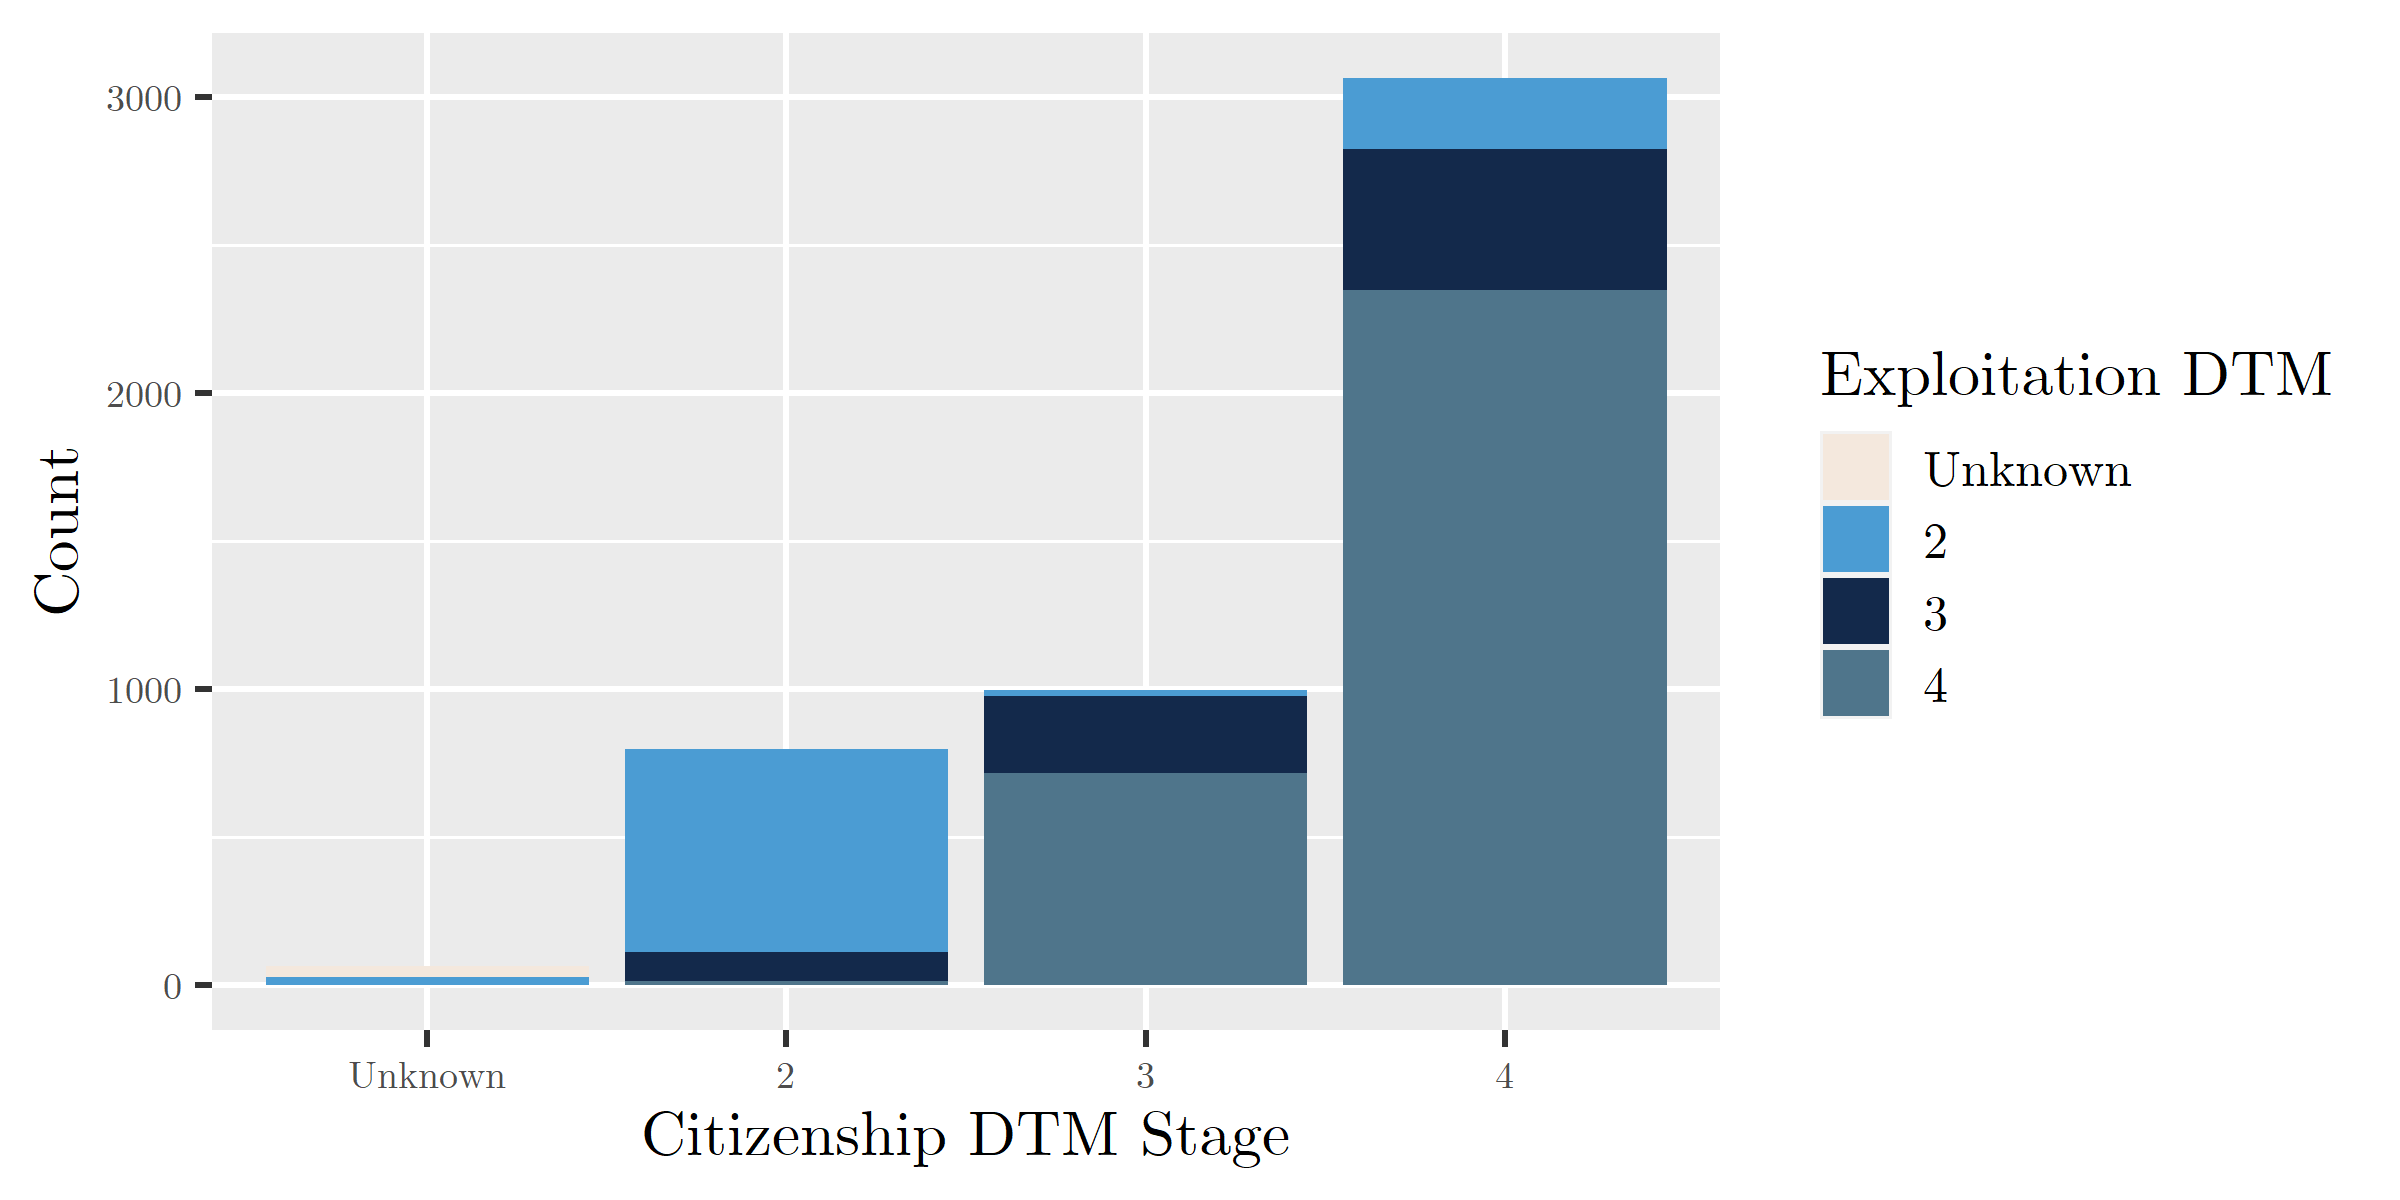
\includegraphics[width = \textwidth]{Different_CountryDTM}
\end{figure}
\FloatBarrier

This image displays a different outcome. Victims from stage 4 countries are more likeley to be exploited in a stage 5 country if they are exploited in a country that is different than their citizenship. However, stages 3 and 5 exhibit the same behavior as before, and all of the stage 2 citizens are exploited in countries in stages 3, 4, and 5. Since there is such a large difference between these two visuals, it means that cases in which the citizenship and exploitation country will lead to substantial multicollinearity in the data, meaning that using both variables in any model we create could prove to be ineffective. 

Additionally, sine the aim of these models is to inform policy makers, it would make sense to use exploitation DTM stage as the variable of choice, since these correspond to the place sin which individuals are actually exploited. However, removing citizenship DTM would remove valuable information for law makers of where the victims in their country are coming from. Some potential ways to counteract this is by assigning a small weight to the citizenship DTM variable, to prevent it from overpowering the rest of the variables in the model. Additionally, adding some random variation to citizenship DTM in our models would lead to the model being more robust. This idea also would be beneficial as it would account for random variation in how DTM stage was determined. Since population pyramids are constantly changing, it is possible there are disagreements on the true DTM classification of a country. For our purposes, each DTM stage in citizenship DTM will either be increased by 1, decreased by 1, or stay the same, with probabilities that will be determined later.

\subsection{Correlation}

Another metric that will help determine the suitability of the data set is by observing the correlation matrix of all variables. In this matrix, darker squares indicate a stronger correlation between two variables. Places in which the squares are lightest indicate little or no correlation. 

\FloatBarrier
\begin{figure}[H]
	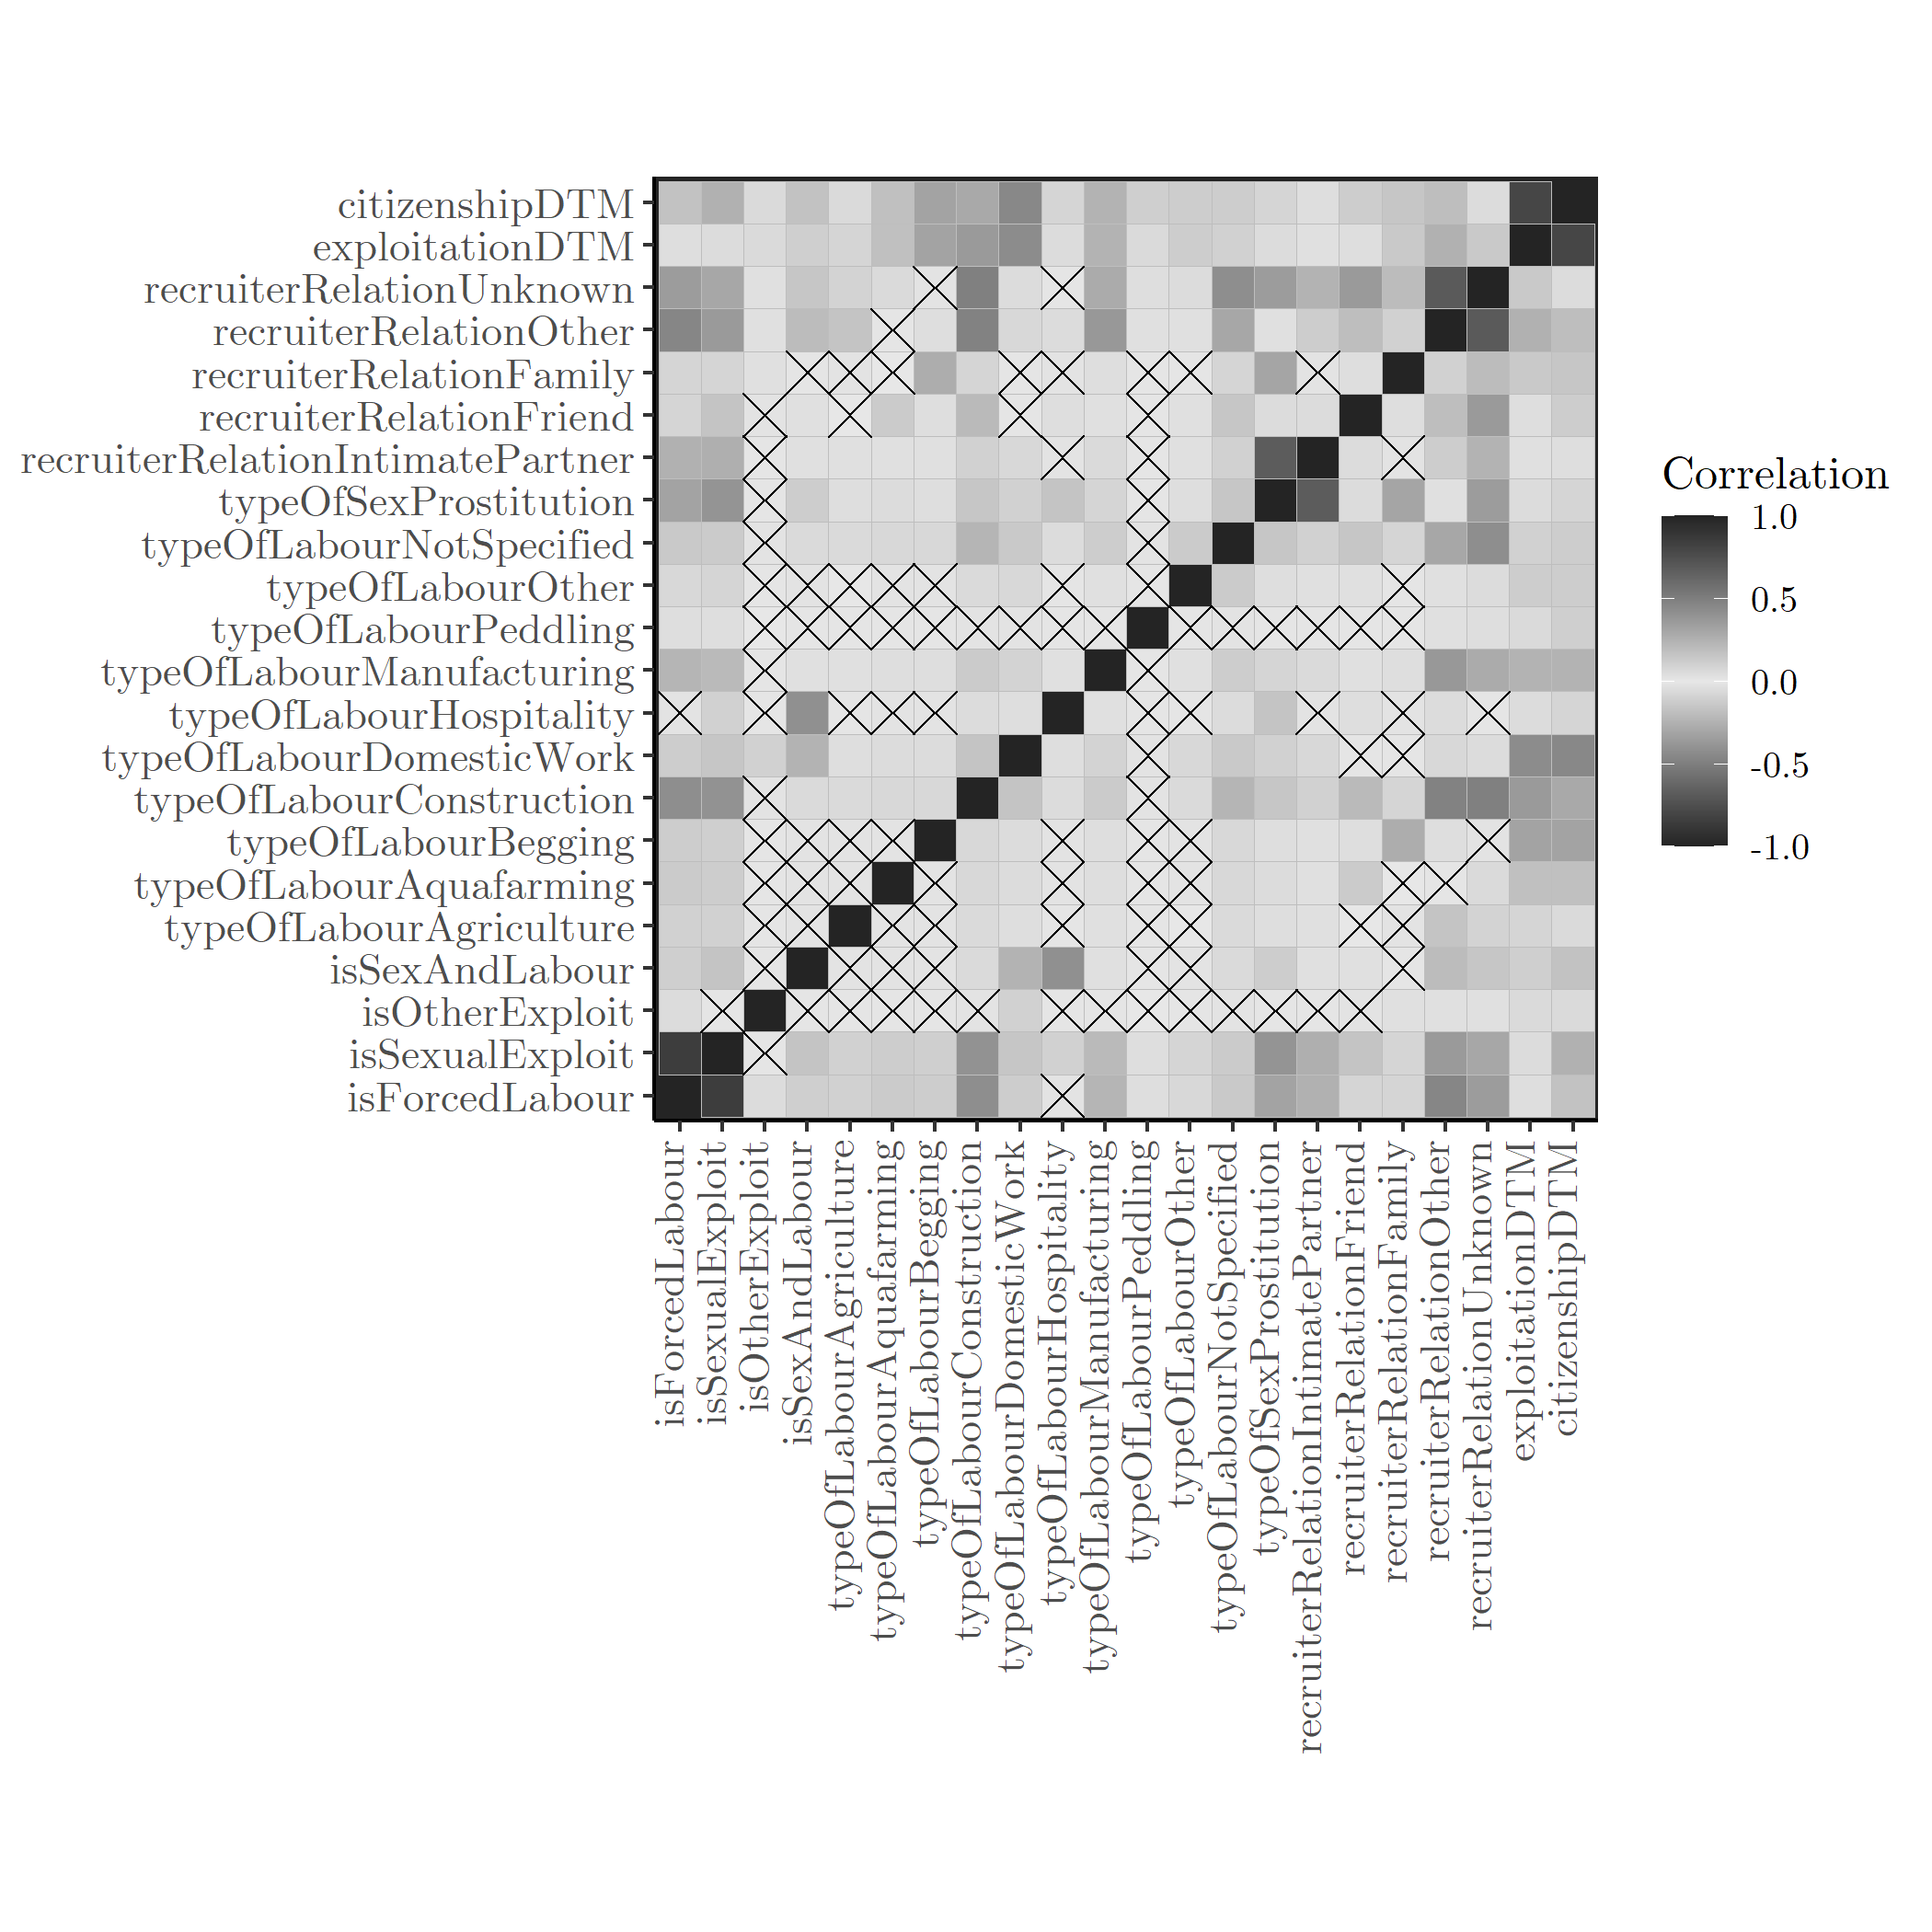
\includegraphics[width = \textwidth]{CorrPlot}
\end{figure}
\FloatBarrier





\printbibliography

\end{document}
